\chapter{QMDD}\label{chap:qmdd}

{\itshape Quantum Multiple-Valued Decision Diagram} é uma estrutura de dados composta de um grafo dirigido acíclico cujos vértices são rotulados a partir de um dos qubits do circuito. Por meio dessas informações, é possível percorrer o grafo de forma a reconstruir completamente a matriz que ele representa. Assim, o QMDD se mostra uma forma sem perdas de compactar matrizes. Além disso, é possível manipular QMDDs e realizar operações como adição e multiplicação entre eles sem precisar reconstruir suas matrizes, fazendo com que essas operações também tirem vantagem da capacidade de compressão oferecida pela estrutura. \cite{miller2006qmdd}

É importante ressaltar que a compressão oferecida pelo QMDD é limitada pela presença da redundância da matriz representada. A forma como o QMDD funciona é representando de forma concisa o produto tensorial entre múltiplas matrizes, como se fosse apenas a representação linear de quais matrizes fazem parte do produto, sem armazenar todo o resultado. Porém, essa representação não é suficiente para incluir portas controladas, que precisam de múltiplos vértices para representar os diferentes cenários que a porta envolve. Por isso, circuitos com alta taxa de entrelaçamento normalmente geram matrizes com baixa taxa de redundância, fazendo com que o QMDD perca sua eficiência na hora de comprimí-la \cite{kydros2025tutorial}. Dessa forma, o tamanho de um QMDD é variado em relação ao número de qubits, podendo ser constante, caso todos os qubits se encontrem na exata mesma distribuição, ou exponencial, caso muitos qubits estejam entrelaçados entre si.

Como estabelecido na \cref{sec:matrixrep}, para que um circuito quântico possa ser convertido em matrizes para ser simulado, são necessárias 3 operações fundamentais: construção da matriz a partir da porta; multiplicação de matrizes; medição. Nesta seção, serão apresentados os algoritmos necessários para realização dessas operações, em conjunto das subrotinas necessárias para os algoritmos. Por exemplo, a multiplicação de QMDDs faz uso da subrotina de adição de QMDDs.

Além disso, também será feita uma breve introdução ao conceito de grafos, e como eles oferecem formas eficazes de percorrer dados por meio de caminhos, uma funcionalidade essencial para a manipulação e recuperação das informações contidas em QMDDs.

\section{Grafos}\label{sec:graph}

Visto que QMDDs dependem integralmente de grafos, esta seção busca introduzir os conceitos necessários para compreender as definições do QMDD e as restrições necessárias para que um grafo seja válido para um QMDD \cite{jungnickel}

Grafo é o nome dado para estruturas de dados organizadas em elementos e ligações entre esses elementos. Cada elemento do grafo é chamado de vértice e as ligações entre os elementos são chamadas de arestas. Um cenário no qual grafos são úteis, por exemplo, é a representação entre diferentes pontos de ônibus de uma cidade e a existência de uma rota que ligue 2 pontos. Nesse caso, cada ponto de ônibus é um vértice e sempre que exista uma linha de ônibus levando de um ponto A para um ponto B, vai existir uma aresta ligando os vértices A e B. Arestas podem ser representadas como uma tupla com o vértice de saída e o vértice destino da aresta.

O grafo da \cref{fig:graph2nodes} é composto do conjunto de vértices \{A, B\} e do conjunto de arestas \{(A, B)\}.

\begin{figure}[h]
  \centering
  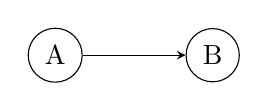
\begin{tikzpicture}[>=stealth, node distance=2cm]

  \node (A) [circle, draw] {A};
  \node (B) [circle, draw, right of=A] {B};

  \draw[->] (A) -- (B);

  \end{tikzpicture}
  \caption{Grafo com 2 vértices}
  \label{fig:graph2nodes}
\end{figure}


\subsection{Caminhos}
A existência de uma aresta saindo de A e levando a B significa que existe um caminho de A para B. Nem todos os vértices do precisam estar diretamente ligados por uma aresta, é possível que exista um caminho indireto entre dois vértices. Por exemplo, no grafo da imagem \cref{fig:graph3node}, existe um caminho de A para B e um de B para C, isso significa que, indiretamente, também existe um caminho de A para C \cite{jungnickel}.

\begin{figure}[h]
  \centering
  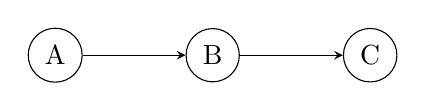
\begin{tikzpicture}[>=stealth, node distance=2cm]

  \node (A) [circle, draw] {A};
  \node (B) [circle, draw, right of=A] {B};
  \node (C) [circle, draw, right of=B] {C};

  \draw[->] (A) -- (B);
  \draw[->] (B) -- (C);

  \end{tikzpicture}
  \caption{Grafo com 3 vértices}
  \label{fig:graph3node}
\end{figure}

\subsection{Arestas Ponderadas}
Além de armazenar apenas a informação de que se existe ou não um caminho entre dois vértices, uma aresta também pode armazenar um valor para esse caminho. Normalmente esse valor é entendido como o custo da aresta, porém, nos QMDDs, esse valor é interpretado como um dos valores que compõem a matriz representada.

No exemplo dos pontos de ônibus, o valor de uma aresta poderia representar o tempo que leva para chegar de um lugar a outro. Isso se torna útil em junção com o conceito de caminho indireto: se o caminho de A para C é na verdade o caminho de A para B seguido do caminho de B para C, sabe-se que o custo para chegar em C a partir de A será a soma dos custos para ir de A a B e de B a C. Por exemplo, se a aresta (A, B) tem valor 10 minutos e a aresta (B, C) tem valor 20 minutos, sabe-se que é possível sair de A e chegar em C em 30 minutos.

\begin{figure}[h]
  \centering
  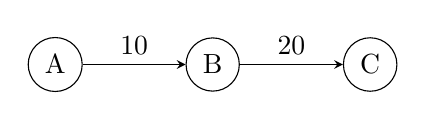
\begin{tikzpicture}[>=stealth, node distance=2cm]

  \node (A) [circle, draw] {A};
  \node (B) [circle, draw, right of=A] {B};
  \node (C) [circle, draw, right of=B] {C};

  \draw[->] (A) -- (B) node[midway, above] {10};
  \draw[->] (B) -- (C) node[midway, above] {20};

  \end{tikzpicture}
  \caption{Grafo com arestas ponderadas}
  \label{fig:graph3nodeweighted}
\end{figure}


\subsection{Grafos Dirigidos e Ciclos}
Note que a possibilidade de ir do ponto A para o ponto B não implica na existência de um caminho de B para A. Por isso a ordem da tupla é importante para as arestas. Dessa forma, grafos podem ou não ser dirigidos, ou seja, é possível impor a restrição de que toda aresta representa a existência de ambos os caminhos, tornando a ordem da tupla irrelevante. Caso o grafo não seja dirigido, toda aresta resulta na existência de um ciclo, ou seja, existe um caminho de um vértice para ele mesmo. No caso da aresta não dirigida (A, B), existe um caminho de A para B e existe um caminho de B para A, logo existe um caminho de A para A.

Por outro lado, no caso de grafos dirigidos, a existência de um ciclo passa a ser apenas uma possibilidade facilmente identificada. No caso dos QMDDs, essa restrição é sempre respeitada pela forma como os algoritmos de construção e manipulação são definidos. Porém, dado um grafo arbitrário, é possivel verificar se existe um ciclo por meio de uma busca a partir de cada vértice, verificando se existe um caminho que leve de volta ao mesmo vértice \cite{jungnickel}.

O presente grafo na \cref{fig:acyclicgraph} é acíclico, visto que não existe caminho de nenhum vértice para si mesmo, já o grafo na \cref{fig:cyclicgraph}, existe um caminho de A para A, passando pelos vértices B e C, logo esse grafo é cíclico.

\begin{figure}[h]
  \centering
  \begin{minipage}{0.45\textwidth}
    \centering
    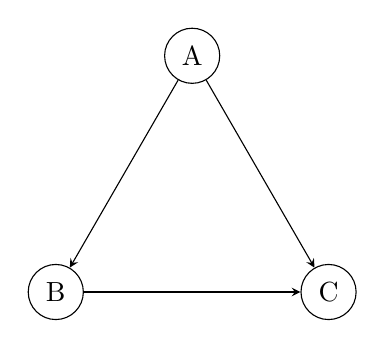
\begin{tikzpicture}[>=stealth, every node/.style={circle,draw,minimum size=7mm}]
      \node (A) at (90:2)  {A};
      \node (B) at (210:2) {B};
      \node (C) at (330:2) {C};
      \draw[->] (A) -- (B);
      \draw[->] (B) -- (C);
      \draw[->] (A) -- (C);
    \end{tikzpicture}
    \caption{Grafo acíclico}
    \label{fig:acyclicgraph}
  \end{minipage}
  \qquad
  \begin{minipage}{0.45\textwidth}
    \centering
    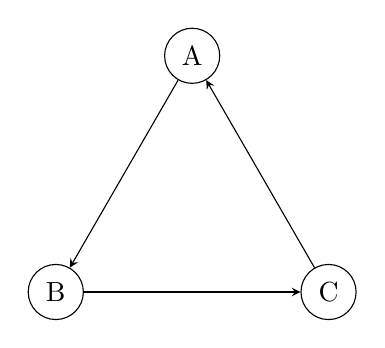
\begin{tikzpicture}[>=stealth, every node/.style={circle,draw,minimum size=7mm}]
      \node (A) at (90:2)  {A};
      \node (B) at (210:2) {B};
      \node (C) at (330:2) {C};
      \draw[->] (A) -- (B);
      \draw[->] (B) -- (C);
      \draw[->] (C) -- (A);
    \end{tikzpicture}
    \caption{Grafo cíclico}
    \label{fig:cyclicgraph}
  \end{minipage}
\end{figure}

\subsection{Representação de Vértices e Arestas}

No começo desta seção, vértices foram apresentadas como sendo elementos arbitrários de um conjunto e arestas como sendo tuplas dos vértices conectados e, opcionalmente, um peso. Para a descrição dos algoritmos do QMDD, uma notação diferente será utilizada. Nela, cada aresta possui apenas um valor e um vértice destino, enquanto cada vértice será uma tupla com seu rótulo e um conjunto de arestas.

Assim, o grafo da \cref{fig:graph3nodeweighted} pode ser representado como o conjunto de vértices $\{(A, \{(10, B)\}), (B, \{(20, C)\}), (C, \{\})\}$

\section{Como Ler um QMDD}\label{sec:qmddvis}

A representação gráfica de um QMDD permite a visualização de como um determinado valor da matriz codificada pode ser extraído por meio de um caminho entre o vértice raiz e o vértice terminal. A \Cref{fig:hqmdd} representa a matriz H. QMDDs que representam uma porta sobre um único qubit podem facilmente ser construídos, precisando apenas de um vértice inicial e um terminal, sendo as 4 arestas do vértice inicial os 4 valores presentes em cada posição da matriz. Note que o diagrama foi normalizado de acordo com o algoritmo de normalização apresentado em \cref{alg:normalization}, fazendo com que $\frac{1}{\sqrt{2}}$, o fator em comum a todas as arestas, seja fatorado e colocado na aresta raiz do diagrama.

\begin{figure}[h]
  \centering
  \begin{tikzpicture}[
    node distance=1.5cm,
    root/.style={circle,draw,minimum size=8mm},
    leaf/.style={rectangle,draw,minimum size=6mm},
    baseline={(current bounding box.center)}
  ]
    % terminal node
    \node[leaf] (t) at (0,0) {$1$};

    % nodes
    \node[root] (v) at (0,2) {q0};

    % incoming edge of weight 1
    \node[above=of v] (src) {};
    \draw[->] (src) -- node[right] {$\frac{1}{\sqrt{2}}$} (v);

    \draw[->] (v) edge[bend left=30]  node[right]  {$1$} (t);
    \draw[->] (v) edge[bend right=30] node[right] {$1$} (t);
    \draw[->] (v) edge[bend left=90]  node[right]  {$-1$} (t);
    \draw[->] (v) edge[bend right=90] node[right] {$1$} (t);
  \end{tikzpicture}
  \caption{QMDD representando a porta de Hadamard.}
  \label{fig:hqmdd}
\end{figure}

Já para matrizes que representam portas sobre múltiplos qubits, a ligação direta entre arestas e posições da matriz deixa de existir. Por exemplo, a matriz $X \otimes H$ pode ser representada com apenas 8 arestas, apesar de ser uma matriz com 16 posições, como demonstrado na \cref{fig:xhqmdd}.

\begin{figure}[h]
  \centering
  \begin{tikzpicture}[
    node distance=1.5cm,
    root/.style={circle,draw,minimum size=8mm},
    leaf/.style={rectangle,draw,minimum size=6mm},
    baseline={(current bounding box.center)}
  ]

    % terminal node
    \node[leaf] (t) at (0,0) {$1$};

    % nodes
    \node[root] (v) at (0,4) {q1};
    \node[root] (B) at (0,2) {q0};


    % incoming edge of weight 1
    \node[above=of v] (src) {};
    \draw[->] (src) -- node[right] {$\frac{1}{\sqrt{2}}$} (v);

    % four outgoing edges, one for each matrix entry (1,0,0,1)
    \draw[->] (v) edge[bend left=90]  node[right]  {$0$} (B);
    \draw[->] (v) edge[bend left=30]  node[right]  {$1$} (B);
    \draw[->] (v) edge[bend right=30] node[right] {$1$} (B);
    \draw[->] (v) edge[bend right=90] node[right] {$0$} (B);

    \draw[->] (B) edge[bend left=30]  node[right]  {$1$} (t);
    \draw[->] (B) edge[bend right=30] node[right] {$1$} (t);
    \draw[->] (B) edge[bend left=90]  node[right]  {$-1$} (t);
    \draw[->] (B) edge[bend right=90] node[right] {$1$} (t);


  \end{tikzpicture}
  \caption{QMDD representando uma porta X aplicada no primeiro qubit e uma porta H no segundo qubit de um circuito}
  \label{fig:xhqmdd}
\end{figure}

Para reconstruir a matriz representada por esse diagrama, basta seguir o caminho da aresta inicial ao vértice final. Cada vértice é rotulado por um qubit e suas arestas representam uma das 4 possíveis escolha para ler o qubit: começou em 0 e está em 0; começou em 0 e está em 1; começou em 1 e está em 0 ou começou em 1 e está em 1. Como os qubits normalmente são inicializados em \ket{0}, pode-se construir o caminho considerando apenas a primeira e a segunda aresta do vértice. Caso o qubit do vértice esteja em \ket{0} no estado a ser lido, segue a primeira aresta e caso esteja em \ket{1} segue a segue.

Uma forma mais algorítmica para recuperar um determinado valor da matriz é construir o caminho a partir dos índices do valor na matriz. Por exemplo, para obter o valor $M_{31}$ (valor na quarta linha e segunda coluna da matriz), é preciso escrever o índice em binário utilizando o número de bits igual ao número de qubits indicado pelo diagrama, no caso (3, 1) vira (11, 01). Então, para escolher a aresta do i-ésimo vértice, monta-se o par linha, coluna do i-ésimo bit mais significativo do índice. Ou seja, no qubit 0, a aresta escolhida será terceira (índice $2_{10}$, ou $10_2$) e a aresta do qubit 1 será a quarta (índice $3_{10}$, ou $11_2$).

Ao atingir o vértice terminal, basta multiplicar os pesos de todas as arestas presentes no caminho tomado para recuperar o valor representado pela matriz original.

\begin{equation}
  M_{31} = \frac{1}{\sqrt{2}} \cdot 1 \cdot -1 = -\frac{1}{\sqrt{2}}
\end{equation}

Note que, na \cref{fig:xhqmdd}, as arestas de $q1$ com peso 0 levam ao vértice $q0$ para facilitar a visualização do grafo. Uma otimização importante é que toda aresta de peso 0 pode levar diretamente ao vértice terminal, já que a presença de um 0 no caminho faz com que o resultado seja 0 independentemente de quais outros valores estiverem presentes.

Outras restrições para que o grafo do QMDD seja construído de forma otimizada são:

\begin{enumerate}
  \item Existe um único vértice que não possui arestas saintes. Esse vértice é chamado de vértice terminal.
  \item Todos os vértices que não são o vértice terminal possuem um rótulo indicando qual qubit o vértice representa e um conjunto de $r^2$ arestas saintes. \cite{fujita1997multi} No caso de QMDDs para circuitos quânticos, $r=2$, logo cada vértice possui 4 arestas.
  \item Existe uma única aresta sem vértice de origem. Essa é a aresta pela qual se iniciam todas as buscas pelo grafo e aponta para o vértice chamado de inicial.
  \item Todas as arestas do grafo são ponderadas por um valor complexo.
  \item Os rótulos dos vértices são ordenáveis, de forma que os rótulos de todo caminho formado do vértice inicial ao terminal estejam ordenados. Ou seja, em uma busca pelo gráfico, sempre se encontrará os vértices de cada qubit na mesma ordem. Além disso, essa ordem diz que o qubit menos significativo do circuito é o mais próximo do vértice terminal, enquanto o mais significativo é o próprio vértice inicial.
  \item Nenhum vértice não terminal é redundante. Ou seja, nenhum vértice possui todas as suas arestas com mesmo peso e apontando para um mesmo vértice. Caso todas as arestas tenham peso 0, o vértice ainda é considerado redundante mesmo que os vértices destino sejam diferentes. Isso porque a presença de um 0 no caminho entre o vértice inicial e final anula inteiramente o valor do caminho, fazendo com que qualquer aresta com peso 0 possa levar imediatamente ao vértice terminal sem alterar o valor do QMDD.
  \item Todo nodo não terminal é sempre normalizado, de forma que a primeira aresta de valor não nulo tem sempre valor 1. Note que deve sempre existir pelo menos uma aresta não nula, pois se todas as arestas tiverem peso 0, o vértice seria redundante.
  \item Todos os vértices são únicos. Ou seja, não existe um par de vértices com mesmo rótulo e todas as arestas iguais.
\end{enumerate}

\subsection{QMDD para vetor de estados}\label{sub:qmddvec}

Para a maior parte do processo de simulação, a principal utilidade do QMDD é para a representação de matrizes. Porém, também é possível utilizá-los para representar vetores e, no contexto da simulação quântica, um vetor de estados. Uma extensão útil do entendimento da representação de um circuito por meio de QMDDs é a de que cada vértice representa uma transformação sobre um dos qubits do circuito. Das 4 arestas do vértice, as duas primeiras indicam o resultado da transformação caso o qubit tenha sido inicializado em \ket{0} e as últimas duas arestas caso o estado inicial do qubit fosse \ket{1}. Dessa forma, escolher quais arestas considerar de acordo com a inicialização o circuito. Tipicamente, todos os qubits do circuito são inicializados em \ket{0} e este trabalho considerará esse o caso padrão para os próximos exemplos. Ou seja, para obter o QMDD que representa o vetor de estados resultante da simulação de um circuito quântico, basta descartar as duas últimas arestas de cada vértice

Por exemplo, o QMDD da \cref{fig:xhqmdd} representa um circuito no qual a porta X foi aplicada sobre o primeiro qubit e a porta H sobre o segundo. Ao ignorar a terceira e a quarta aresta de cada vértice deste grafo, resta o QMDD presente na \cref{fig:xhqmddresult}.

\begin{equation}
  \begin{tikzpicture}[
    node distance=1.5cm,
    root/.style={circle,draw,minimum size=8mm},
    leaf/.style={rectangle,draw,minimum size=6mm},
    baseline={(current bounding box.center)}
  ]

    % terminal node
    \node[leaf] (t) at (0,0) {$1$};

    % nodes
    \node[root] (v) at (0,4) {q1};
    \node[root] (B) at (0,2) {q0};


    % incoming edge of weight 1
    \node[above=of v] (src) {};
    \draw[->] (src) -- node[right] {$\frac{1}{\sqrt{2}}$} (v);

    \draw[->] (v) edge[bend right=30] node[left] {$0$} (B);
    \draw[->] (v) edge[bend left=30] node[right] {$1$} (B);

    \draw[->] (B) edge[bend right=30] node[left] {$1$} (t);
    \draw[->] (B) edge[bend left=30] node[right] {$1$} (t);

  \end{tikzpicture}
  \label{fig:xhqmddresult}
\end{equation}

Para obter o valor de cada estado, basta percorrer o grafo seguindo as arestas de acordo com o estado desejado. Por exemplo, para obter o valor do estado \ket{00}, basta seguir a aresta esquerda do primeir qubit e a aresta direita do segundo qubit e multiplicar todos os pesos encontrados.

\begin{equation}
  \frac{1}{\sqrt{2}} * 0 * 1 = 0
\end{equation}

Logo, o estado $\ket{\psi}$ obtido com a execução do circuito pode ser reconstruído percorrendo cada um dos possíveis caminhos, como na equação a seguir:

\begin{equation}
  \ket{\psi}
  =
  \textcolor{blue}{\frac{1}{\sqrt{2}} \cdot 0 \cdot 1} \cdot \ket{00}
  +
  \textcolor{blue}{\frac{1}{\sqrt{2}} \cdot 0 \cdot 1} \cdot \ket{01}
  +
  \textcolor{blue}{\frac{1}{\sqrt{2}} \cdot 1 \cdot 1} \cdot \ket{10}
  +
  \textcolor{blue}{\frac{1}{\sqrt{2}} \cdot 1 \cdot 1} \cdot \ket{11}
  =
  \textcolor{blue}{\frac{1}{\sqrt{2}}} \cdot (\ket{10} + \ket{11})
\end{equation}

\section{Algoritmos}

A seguir, serão definidas operações entre arestas de QMDDs. Dessa forma, a operação entre dois QMDDs é realizada por meio da operação entre suas duas arestas iniciais.

A maior parte das operações são construídas de forma recursiva. Isso significa que o algoritmo é divido em dois passos: o inicial e o recursivo. O passo inicial representa um cenário trivial, no qual a solução pode ser facilmente encontrada, já o passo recursivo pode ser entendido como uma combinação de múltiplos passos iniciais, nele é preciso definir como os passos iniciais serão construídos e como seus resultados serão utilizados para gerar o resultado do passo recursivo.

Para o QMDD, o passo inicial é quando se atinge uma aresta terminal, fazendo com que a operação normalmente se resuma a aplicar a mesma operação sobre o peso das arestas. Já o passo recursivo acontece sobre arestas não terminais, que dependem do resultado da operação entre as arestas dos vértices que as arestas de entrada apontam. 

\subsection{Funções Fundamentais}\label{sub:fundamentals}

Para definição sucinta dos algoritmos, serão utilizadas algumas notações para se referir a informações presentes nos vértices e arestas do QMDD.

\begin{enumerate}
  \item $x(v)$: $v$ é um vértice e $x(v)$ signfica o rótulo do vértice $v$;
  \item $v(e)$: $e$ é uma aresta e $v(e)$ representa o vértice ao qual a aresta aponta;
  \item $w(e)$: $e$ é uma aresta e $w(e)$ é o peso dessa aresta;
  \item $E_i(x)$: Quando $x$ é um vértice, $E_i(x)$ é a i-ésima aresta do vértice. Quando $x$ é uma aresta, $E_i(x)$ é a i-ésima aresta do vértice ao qual $x$ aponta;
  \item $T(e)$: $e$ é uma aresta e $T(e)$ é um valor verdadeiro ou falso que indica se a aresta é terminal. Ou seja, se o vértice ao qual $e$ aponta é o vértice terminal;
  \item $v_t$: é o vértice terminal do QMDD, que não contém nenhuma aresta.

\end{enumerate}


Além disso, note que, para representar as matrizes utilizadas por circuitos quânticos, o número de arestas por vértice do QMDD será sempre 4. Apesar de ser possível que diferentes usos de matrizes requeiram diferentes números de arestas por vértice, os algoritmos serão descritos com os valores fixos para as matrizes relevantes para a simulação de circuitos quânticos.

\subsection{Normalização e Eliminação de Redundância}

Normalizar um vértice é essencial para possibilitar a detecção de redundância presente em um QMDD, visto que a presença de um múltiplo em comum a todas as arestas de um mesmo vértice pode ser fatorado e adicionado à aresta que aponta para esse vértice. Dessa forma, a equivalência entre diferentes vértices pode ser encontrada apenas comparando o alvo e peso de suas arestas.

O processo de normalizar um vértice também envolve a remoção de vértices reduntantes. Ou seja, vértices cujas arestas sejam todas iguais entre si podem ser substituídos por um caminho direto para o alvo de suas arestas. Assim, o algoritmo de normalização deve retornar uma aresta que aponta ou para o vértice original (caso o vértice não seja redundante) ou para o próximo vértice (caso o original seja reduntante). Por isso, é importante que os algoritmos sejam definidos sobre as arestas e não sobre os vértices. Assim, para normalizar um vértice, o algoritmo deve ser aplicado sobre a aresta que aponta para esse vértice.

Além disso, como as outras operações constroem seu resultado do vértice final ao inicial, o fato que o algoritmo de normalização retorna a aresta que aponta para o vértice faz com que o efeito da normalização seja propagado do vértice final ao inicial. 

O algoritmo em si se divide em duas etapas: primeiro verifica-se se o vértice é redundante e, se não for, normaliza-se os pesos de suas arestas.

As linhas 1 e 2 do \cref{alg:normalization} identificam a redundância do vértice, basta comparar todas as suas arestas. Se todas forem iguais (mesmo peso e mesmo vértice alvo), o vértice pode ser descartado, então basta retornar uma aresta com o alvo das arestas do vértice e o peso sendo o produto de uma dessas arestas com o da de entrada.

Caso o vértice não seja redundante, o peso de todas as suas arestas será dividido pelo peso da primeira aresta com peso diferente de 0. As linhas 3 a 13 do \cref{alg:normalization} realizam essa tarefa. As linhas 5 e 6 ignoram arestas nulas, as linhas 3, 7 e 8 identificam o peso da primeira aresta não nula. E nas linhas 11 e 12 os pesos das arestas são normalizados, as arestas do vértice têm seus pesos divididos pelo valor identificado como peso da primeira aresta não nula, enquanto a aresta de entrada do algoritmo tem seu peso multiplicado por esse valor.  

Isso faz com que todo vértice tenha sua primeira aresta não nula com peso 1. Então, basta retornar uma nova aresta, apontando para o mesmo vértice e com peso sendo o peso original multiplicado pelo fator em comum às arestas do vértice \cite{miller2006qmdd}.

\begin{algorithm}[H]
  \caption{Normalização de Vértice da Aresta}
  \label{alg:normalization}
  \KwIn{Aresta $e$}
  \KwOut{Aresta}

  \If{$E_0(e) = E_1(e) = E_2(e) = E_3(e)$}{
    \Return $Aresta(w(e)*w(E_0(e)), v(E_0(e))$)
  }
  $w \gets 0$ \;
  \For{$i \gets 0$ \KwTo $3$}{
    \If{$w(E_i(e)) = 0$}{
      \KwContinue
    }
    \If{$w = 0 $}{
      $w \gets w(E_i(e))$
    }
    \If{$w \neq 0 $}{
      $w(E_i) \gets w(E_i(e) / w $)
    }
  
  $w(E_i(e)) \gets w(E_i(e))/w$
  }

  $w(e) \gets w * w(e) $

  \Return $e$

\end{algorithm}

A seguir, são oferecidos dois exemplos de normalização de vértices. Na cref{fig:redundantNormalization}, o vértice é reduntante pois todas suas arestas são iguais, logo é descartado e o fator comum a todas as arestas é passado para a aresta de entrada. Já na \cref{fig:exampleNormalization}, a primeira aresta é ignorada por ter peso 0, enquanto as demais tem seus pesos dividos pelo peso da primeira aresta não nula, que é 2. Por fim, o peso da aresta de entrada é multiplicado por 2.

\begin{figure}[H]
  \centering
  \begin{tikzpicture}[
    node distance=1.5cm,
    root/.style={circle,draw,minimum size=8mm},
    leaf/.style={rectangle,draw,minimum size=6mm},
    baseline={(current bounding box.center)}
  ]

    \node[leaf] (t) at (0,0) {$1$};
    \node[root] (v) at (0,2) {};

    \node[above=of v] (src) {};
    \draw[->] (src) -- node[right] {$1$} (v);

    \draw[->] (v) edge[bend right=90] node[right] {$\frac{1}{2}$} (t); % (1,1)
    \draw[->] (v) edge[bend right=30] node[right] {$\frac{1}{2}$} (t); % (1,0)
    \draw[->] (v) edge[bend left=30]  node[right]  {$\frac{1}{2}$} (t); % (0,1)
    \draw[->] (v) edge[bend left=90]  node[right]  {$\frac{1}{2}$} (t); % (0,0)

  \end{tikzpicture}
  $\quad\Longrightarrow\quad$
  \begin{tikzpicture}[
    node distance=1.5cm,
    root/.style={circle,draw,minimum size=8mm},
    leaf/.style={rectangle,draw,minimum size=6mm},
    baseline={(current bounding box.center)}
  ]

    % terminal node
    \node[leaf] (t) at (0,0) {$1$};

    % incoming edge of weight 1
    \node[above=of t] (src) {};
    \draw[->] (src) -- node[right] {$\frac{1}{2}$} (t);

  \end{tikzpicture}
  \caption{Normalização de um vértice reduntante}
  \label{fig:redundantNormalization}
\end{figure}

\begin{figure}[H]
  \centering
  \begin{tikzpicture}[
    node distance=1.5cm,
    root/.style={circle,draw,minimum size=8mm},
    leaf/.style={rectangle,draw,minimum size=6mm},
    baseline={(current bounding box.center)}
  ]

    \node[leaf] (t) at (0,0) {$1$};
    \node[root] (v) at (0,2) {};

    \node[above=of v] (src) {};
    \draw[->] (src) -- node[right] {$1$} (v);

    \draw[->] (v) edge[bend right=90] node[right] {$0$} (t); % (1,1)
    \draw[->] (v) edge[bend right=30] node[right] {$2$} (t); % (1,0)
    \draw[->] (v) edge[bend left=30]  node[right]  {$1$} (t); % (0,1)
    \draw[->] (v) edge[bend left=90]  node[right]  {$1$} (t); % (0,0)

  \end{tikzpicture}
  $\quad\Longrightarrow\quad$
  \begin{tikzpicture}[
    node distance=1.5cm,
    root/.style={circle,draw,minimum size=8mm},
    leaf/.style={rectangle,draw,minimum size=6mm},
    baseline={(current bounding box.center)}
  ]

    \node[leaf] (t) at (0,0) {$1$};
    \node[root] (v) at (0,2) {};

    \node[above=of v] (src) {};
    \draw[->] (src) -- node[right] {$2$} (v);

    \draw[->] (v) edge[bend right=90] node[right] {$0$} (t); % (1,1)
    \draw[->] (v) edge[bend right=30] node[right] {$1$} (t); % (1,0)
    \draw[->] (v) edge[bend left=30]  node[right]  {$\frac{1}{2}$} (t); % (0,1)
    \draw[->] (v) edge[bend left=90]  node[right]  {$\frac{1}{2}$} (t); % (0,0)

  \end{tikzpicture}

  \caption{Normalização de um vértice não reduntante}
  \label{fig:exampleNormalization}
\end{figure}


\subsection{Adição}

Apesar de não ser uma operação diretamente necessária para simulação de circuitos, a adição de matrizes é um passo essencial para a multiplicação de matrizes, que, por sua vez, é necessária para a simulação.

Caso pelo menos uma das arestas a serem somadas seja uma aresta terminal, basta somar o peso da aresta terminal ao peso da outra aresta. As linhas 1 a 8 do \cref{alg:addition} realizam essa parte do algoritmo. Nas linhas 1 e 2, verifica-se se pelo menos uma das duas arestas a serem somadas é terminal, e a identifica como $e_0$. Então as linhas 3 a 8 retornam uma nova aresta cujo peso é a soma dos pesos das duas arestas e o alvo é o alvo da aresta não terminal (se somente uma for terminal, caso ambas sejam terminais o alvo é o vértice terminal).

Caso nenhuma aresta seja terminal, isso significa que as duas arestas apontam para algum vértice que, por sua vez, possui outras 4 arestas. O resultado da soma das duas arestas deve ser um vértice cujas vértices sejam as somas dos 4 pares de arestas que os vértices possuem. Isso é feito nas linhas 9 a 13 do \cref{alg:addition}. A linha 9 cria um vértice sem arestas e o laço de repetição das linhas 11 a 13 cria cada uma das arestas desse vértice \cite{miller2006qmdd}.

Para os próximos algoritmos, é importante que, sempre que um vértice novo seja criado, ele seja normalizado. Isso pois a operação entre dois vértices normalizados não retorna garantidamente um vértice normalizado. Na \cref{fig:exampleAddition} é oferecido um exemplo de adição no qual isso acontece.

\begin{algorithm}[H]
  \caption{Adição de Arestas}
  \label{alg:addition}
  \KwIn{Aresta $e_0$, Aresta $e_1$}
  \KwOut{Aresta}

  \If{$T(e_1)$}{
    $e_0, e_1 \gets e_1, e_0$
  }
  \If{$T(e_0)$}{
    \If{$w(e_0) = 0$}{
      \Return $e_1$
    }
    \If{$T(e_0)$}{
      $e_n \gets Aresta(w(e_0)+w(e_1), v(e_0))$ \;
      \Return $e_n$
    }
  }
  $v_n \gets Vertice(x(e_0), \emptyset)$ \;
  \For{$i \gets 0$ \KwTo $3$}{
    $p \gets Aresta(w(e_0)*w(E_i(e_0)), v(E_i(e_0)))$ \;
    $q \gets Aresta(w(e_1)*w(E_i(e_1)), v(E_i(e_1)))$ \;
    $E_i(v_n) \gets p + q$
  }
  \Return $normalize(Aresta(1, v_n))$

\end{algorithm}

Na \cref{fig:exampleAddition}, são somados dois QMDDs, o primeiro representa a matriz $\begin{bmatrix}1 & 0 \\ 0 & 1\end{bmatrix}$ enquanto o segundo representa a matriz $\begin{bmatrix}0 & 1 \\ 1 & 0\end{bmatrix}$. As arestas de entrada da operação são as arestas iniciais de cada QMDD. Como elas não são terminais, é preciso somar as arestas dos vértices aos quais elas apontam. Assim, a primeira aresta de $q0$ é somada com a primeira aresta de $q1$ e assim sucessivamente.O resultado dessa soma é $\begin{bmatrix}1 & 1 \\ 1 & 1\end{bmatrix}$ e o vértice resultante é reduntante, logo é descartado na etapa de normalização.

\begin{equation}
  \label{fig:exampleAddition}
  \begin{tikzpicture}[
    node distance=1.5cm,
    root/.style={circle,draw,minimum size=8mm},
    leaf/.style={rectangle,draw,minimum size=6mm},
    baseline={(current bounding box.center)}
  ]

    % terminal node
    \node[leaf] (t) at (0,0) {1};

    % QMDD internal node
    \node[root] (v) at (0,2) {};

    % incoming edge of weight 1
    \node[above=of v] (src) {};
    \draw[->] (src) -- node[right] {1} (v);

    % TODO: Use better colors
    % four outgoing edges, one for each matrix entry (1,0,0,1)
    \draw[->, draw=red] (v) edge[bend left=90]  node[right]  {1} (t);
    \draw[->, draw=blue] (v) edge[bend left=30]  node[right]  {0} (t);
    \draw[->, draw=green] (v) edge[bend right=30] node[right] {0} (t);
    \draw[->, draw=orange] (v) edge[bend right=90] node[right] {1} (t);

  \end{tikzpicture}
  \;+\;
  \begin{tikzpicture}[
    node distance=1.5cm,
    root/.style={circle,draw,minimum size=8mm},
    leaf/.style={rectangle,draw,minimum size=6mm},
    baseline={(current bounding box.center)}
  ]

    \node[leaf] (t) at (0,0) {1};
    \node[root] (v) at (0,2) {};

    \node[above=of v] (src) {};
    \draw[->] (src) -- node[right] {1} (v);

    \draw[->, draw=red] (v) edge[bend left=90]  node[right]  {0} (t);
    \draw[->, draw=blue] (v) edge[bend left=30]  node[right]  {1} (t);
    \draw[->, draw=green] (v) edge[bend right=30] node[right] {1} (t);
    \draw[->, draw=orange] (v) edge[bend right=90] node[right] {0} (t);

  \end{tikzpicture}
  \;=\;
  \begin{tikzpicture}[
    node distance=1.5cm,
    root/.style={circle,draw,minimum size=8mm},
    leaf/.style={rectangle,draw,minimum size=6mm},
    baseline={(current bounding box.center)}
  ]

    \node[leaf] (t) at (0,0) {1};
    \node[root] (v) at (0,2) {};

    \node[above=of v] (src) {};
    \draw[->] (src) -- node[right] {1} (v);

    \draw[->, draw=red] (v) edge[bend left=90]  node[right]  {1} (t); % (0,0)
    \draw[->, draw=blue] (v) edge[bend left=30]  node[right]  {1} (t); % (0,1)
    \draw[->, draw=green] (v) edge[bend right=30] node[right] {1} (t); % (1,0)
    \draw[->, draw=orange] (v) edge[bend right=90] node[right] {1} (t); % (1,1)

  \end{tikzpicture}
  \quad\Longrightarrow\quad
  \begin{tikzpicture}[
    node distance=1.5cm,
    root/.style={circle,draw,minimum size=8mm},
    leaf/.style={rectangle,draw,minimum size=6mm},
    baseline={(current bounding box.center)}
  ]

    % terminal node
    \node[leaf] (t) at (0,0) {1};

    % incoming edge of weight 1
    \node[above=of t] (src) {};
    \draw[->] (src) -- node[right] {1} (t);

  \end{tikzpicture}
\end{equation}

\subsection{Multiplicação}

O algoritmo de multiplicação de QMDDs segue a mesma lógica da multiplicação de matrizes. São construídas n matrizes cujos valores são a multiplicação da i-ésima posição da linha da primeira e a i-ésima posição da coluna da segunda. Essas matrizes são então somadas para obter o resultado da multiplicação.

Assim como na adição, o passo inicial do algoritmo é quando pelo menos uma das arestas é uma aresta final. As linhas 1 a 8 do \cref{alg:multiplication} seguem a mesma lógica que a adição para verificar se pelo menos uma das arestas é termianl. A diferença é que, agora, em vez de somados, os pesos das arestas são multiplicados. A lógica para escolha de alvo é a mesma da adição.

% TODO: eu tenho quase ctz que a ordem de linha-coluna ta invertida
Caso nenhuma aresta seja terminal, é necessário construir um novo vértice para acumular o resultado da multiplicação das duas arestas. Para cada posição dos pares linha-coluna das arestas do vértice cujas arestas de entrada apontam, é construída uma nova aresta para armazenar o produto do par. O valor da nova aresta é então somado na posição respectiva do novo vértice. No \cref{alg:multiplication}, as linhas 10 e 11 servem para navegar pelos índices das arestas de cada vértice. A linha 12 cria uma aresta representando a linha $i$, coluna $j$ da matriz resultante, enquanto as linhas 13 a 16 fazem a soma dos produtos cada um dos pares ao longo da linha $i$ da primeira matriz com a coluna $j$ da segunda. A construção das duas arestas, nas linhas 14 e 15, envolve multiplicar o peso da aresta de entrada pelo peso da aresta que será utilizada para aplicar o passo recursivo.

\begin{algorithm}[H]
  \caption{Multiplicação de Arestas}
  \label{alg:multiplication}
  \KwIn{Aresta $e_0$, Aresta $e_1$}
  \KwOut{Aresta}

  \If{$T(e_1)$}{
    $e_0, e_1 \gets e_1, e_0$
  }
  \If{$T(e_0)$}{
    \If{$w(e_0) = 0 $}{
      \Return $e_0$
    }
    \If{$w(e_0) = 1$}{
      \Return $e_1$
    }
    \Return $Aresta(w(e_0)*w(e_1), v(e_1))$
  }
  $v_n \gets Vertice(x(e_0), \emptyset)$ \;
  \For{$i \gets 0$ \KwTo $1$}{
    \For{$j \gets 0$ \KwTo $1$}{
      $E_{2*i+j}(v_n) \gets Aresta(0, v_t)$ \;
      \For{$k \gets 0$ \KwTo $1$}{
        $p \gets Aresta(w(e_0)*w(E_{2*i+k(e_0)}), v(E_{2*i+k}(e_0)))$ \;
        $q \gets Aresta(w(e_1)*w(E_{j+2*k(e_0)}), v(E_{j+2*k}(e_1)))$ \;
        $E_{2*i+j}(v_n) \gets E_{2*i+j}(v_n) + p*q$
      }
    }
  }
  $e_n \gets normalize(Aresta(1, v_n))$ \;
  \Return $e_n$

\end{algorithm}

No exemplo a seguir, é realizada a multiplicação entre a matriz H e a X. O resultado deve ser uma matriz que represente a aplicação da porta X seguida da aplicação da porta H sobre um qubit. A matriz que representa essa operação é obtida a partir da seguinte equação:

\begin{equation}
  \label{eq:hx}
  H \cdot X
  =
  \frac{1}{\sqrt{2}}
  \begin{bmatrix}
    1 & 1 \\
    1 & -1
  \end{bmatrix}
  \cdot
  \begin{bmatrix}
    0 & 0 \\
    1 & 1
  \end{bmatrix}
  =
  \frac{1}{\sqrt{2}}
  \begin{bmatrix}
    1 & 1 \\
    -1 & 1
  \end{bmatrix}
\end{equation}

Como as arestas inicias de ambos os QMDDs não são terminais, o produto entre elas precisa calcular o produto entre as arestas dos vértices aos quais elas apontam. Já que $r=2$ para QMDDs que representam portas quânticas, o produto entre duas arestas não terminais pode ser entendido como a soma de duas matrizes, uma para cada posição do par linha-coluna definido pela multiplicação. A fins de implementação, é mais eficiente que cada posição da matriz resultante seja calculada em um único passo, porém, para fins de demonstração, serão calculadas duas matrizes que serão somadas para obter o resultado final.

\begin{equation}
  \label{fig:exampleMultiplication}
  \begin{tikzpicture}[
    node distance=1.5cm,
    root/.style={circle,draw,minimum size=8mm},
    leaf/.style={rectangle,draw,minimum size=6mm},
    baseline={(current bounding box.center)}
  ]

    % terminal node
    \node[leaf] (t) at (0,0) {1};

    % QMDD internal node
    \node[root] (v) at (0,2) {};

    % incoming edge of weight 1
    \node[above=of v] (src) {};
    \draw[->] (src) -- node[right] {$\frac{1}{\sqrt{2}}$} (v);

    % TODO: Use better colors
    % four outgoing edges, one for each matrix entry (1,0,0,1)
    \draw[->] (v) edge[bend right=90] node[right] {1} (t);
    \draw[->] (v) edge[bend right=30] node[right] {1} (t);
    \draw[->] (v) edge[bend left=30]  node[right]  {1} (t);
    \draw[->] (v) edge[bend left=90]  node[right]  {-1} (t);

  \end{tikzpicture}
  \;\cdot\;
  \begin{tikzpicture}[
    node distance=1.5cm,
    root/.style={circle,draw,minimum size=8mm},
    leaf/.style={rectangle,draw,minimum size=6mm},
    baseline={(current bounding box.center)}
  ]

    \node[leaf] (t) at (0,0) {1};
    \node[root] (v) at (0,2) {};

    \node[above=of v] (src) {};
    \draw[->] (src) -- node[right] {1} (v);

    \draw[->] (v) edge[bend right=90]  node[right]  {0} (t);
    \draw[->] (v) edge[bend right=30]  node[right]  {1} (t);
    \draw[->] (v) edge[bend left=30] node[right] {1} (t);
    \draw[->] (v) edge[bend left=90] node[right] {0} (t);

  \end{tikzpicture}
  \;=\;
  \begin{tikzpicture}[
    node distance=1.5cm,
    root/.style={circle,draw,minimum size=8mm},
    leaf/.style={rectangle,draw,minimum size=6mm},
    baseline={(current bounding box.center)}
  ]

    \node[leaf] (t) at (0,0) {1};
    \node[root] (v) at (0,2) {};

    \node[above=of v] (src) {};
    \draw[->] (src) -- node[right] {1} (v);

    \draw[->] (v) edge[bend right=90]  node[right]  {0} (t); % (0,0)
    \draw[->] (v) edge[bend right=30]  node[right]  {0} (t); % (0,1)
    \draw[->] (v) edge[bend left=15] node[right] {$\frac{1}{\sqrt{2}}$} (t); % (1,0)
    \draw[->] (v) edge[bend left=90] node[right] {$\frac{1}{\sqrt{2}}$} (t); % (1,1)

  \end{tikzpicture}
  \;+\;
  \begin{tikzpicture}[
    node distance=1.5cm,
    root/.style={circle,draw,minimum size=8mm},
    leaf/.style={rectangle,draw,minimum size=6mm},
    baseline={(current bounding box.center)}
  ]

    \node[leaf] (t) at (0,0) {1};
    \node[root] (v) at (0,2) {};

    \node[above=of v] (src) {};
    \draw[->] (src) -- node[right] {1} (v);

    \draw[->] (v) edge[bend right=90]  node[right]  {$\frac{1}{\sqrt{2}}$} (t); % (0,0)
    \draw[->] (v) edge[bend right=20]  node[right]  {$\frac{-1}{\sqrt{2}}$} (t); % (0,1)
    \draw[->] (v) edge[bend left=40] node[right] {0} (t); % (1,0)
    \draw[->] (v) edge[bend left=90] node[right] {0} (t); % (1,1)

  \end{tikzpicture}
  \quad\Longrightarrow\quad
  \begin{tikzpicture}[
    node distance=1.5cm,
    root/.style={circle,draw,minimum size=8mm},
    leaf/.style={rectangle,draw,minimum size=6mm},
    baseline={(current bounding box.center)}
  ]

    \node[leaf] (t) at (0,0) {1};
    \node[root] (v) at (0,2) {};

    \node[above=of v] (src) {};
    \draw[->] (src) -- node[right] {$\frac{1}{\sqrt(2)}$} (v);

    \draw[->] (v) edge[bend right=90]  node[right]  {1} (t); % (0,0)
    \draw[->] (v) edge[bend right=30]  node[right]  {-1} (t); % (0,1)
    \draw[->] (v) edge[bend left=30] node[right] {1} (t); % (1,0)
    \draw[->] (v) edge[bend left=90] node[right] {1} (t); % (1,1)

  \end{tikzpicture}
\end{equation}

Esta representação é equivalente a calcular o produto das matrizes pela seguinte equação:

\begin{equation}
  \label{eq:hx}
  H \cdot X
  =
  \frac{1}{\sqrt{2}}
  \begin{bmatrix}
    1 & 1 \\
    1 & -1
  \end{bmatrix}
  \cdot
  \begin{bmatrix}
    0 & 1 \\
    1 & 0
  \end{bmatrix}
  =
  \begin{bmatrix}
    0 & \frac{1}{\sqrt{2}} \\
    0 & \frac{1}{\sqrt{2}}
  \end{bmatrix}
  +
  \begin{bmatrix}
    \frac{1}{\sqrt{2}} & 0 \\
    \frac{-1}{\sqrt{2}} & 0
  \end{bmatrix}
  =    
  \frac{1}{\sqrt{2}}
  \begin{bmatrix}
    1 & 1 \\
    -1 & 1
  \end{bmatrix}
\end{equation}

\subsection{Construção a Partir de Portas}\label{sec:gateconstruct}

A construção de um QMDD a partir de uma porta quântica pode ser feita de duas formas: uma porta arbitrária para um único qubit ou uma porta arbitrária controlada, com um qubit alvo e múltiplos qubits de controle.

A construção de uma porta arbitrária se dá pelo produto tensorial entre matrizes identidade e a matriz que representa a porta arbitrária, de forma a produzir uma única matriz que opere sobre todos os qubits, mantendo todos exceto o qubit alvo da porta inalterados e aplicando o efeito da porta sobre o qubit desejado. Para isso, basta utilizar o algoritmo de produto tensorial definido na \cref{subsub:kronecker}. Assim, para aplicar uma porta U no i-ésimo qubit de um circuito com k qubits, basta realizar o produto tensorial $I^{\otimes i-1} \otimes U \otimes I^{\otimes k-i}$. 

Já a construção de portas controlodas possui duas etapas: uma para os qubits de controle mais significativos que o qubit alvo e uma para os menos significativos. Essas duas etapas são descritas na \cref{subsub:controlgate} \cite{miller2006qmdd, kydros2025tutorial}

\subsubsection{Produto Tensorial}\label{subsub:kronecker}

O produto tensorial consiste basicamente do encadeamento dos grafos de cada diagrama. $A \otimes B$ significa que as arestas terminais de A serão conectadas ao vértice inicial de B. Note que, por não criar novos vértices, o resultado do produto tensorial não consome mais memória que os dois valores de entrada do produto. Isso representa um ganho exponencial em relação à representação matricial do produto tensorial, cujo tamanho do resultado é o produto dos tamanhos das entradas.

Diferentemente das operações previamente mencionadas, o produto tensorial não avança sobre as duas arestas. Em vez disso, a segunda aresta da operação é levada adiante, de forma que apenas a primeira será alterada. Isso porque a parte mais relevante do produto tensorial acontece entre a aresta inicial do segundo QMDD e todas as arestas finais do primeiro QMDD. Assim, para realizar o produto tensorial, basta percorrer o primeiro QMDD até encontrar suas arestas terminais. Em cada aresta será aplicado o passo de ligar a aresta terminal do primeiro QMDD ao vértice inicial do segundo e a multiplicação dos pesos da aresta final com a aresta inicial.

Além disso, a forma como a navegação do primeiro QMDD é feita faz com que o fator da aresta inicial do segundo QMDD seja propagado até chegar na aresta inicial do primeiro QMDD, por meio do processo sucessivo de normalização das arestas.

As linhas 1 a 6 do \cref{alg:kronecker} representam o momento em que uma aresta terminal do primeiro QMDD é atingida. Nesse caso, a aresta terminal do primeiro grafo deve ser substituída pela aresta inicial do segundo grafo com o peso sendo o produto dos dois pesos. Essa operação é feita na linha 6, as linhas 2 a 5 são otimizações para evitar a rescontrução de arestas desnecessariamente. No caso, caso a aresta terminal tenha peso 0, não é necessário conectar o vértice ao segundo QMDD, pois o peso 0 neste caminho anula quaisquer valores subsequentes. Caso a aresta tenha peso 1, basta substituí-la pela aresta já existente.

As linhas 7 a 9 são responsáveis pela navegação do primeiro QMDD, buscando as arestas terminais e reconstruindo o grafo conforme resultados são obtidos. Por exemplo, na linha 9, a aresta de entrada do segundo QMDD é passada adiante junto de cada aresta do vértice do primeiro QMDD. Note também que, cada vértice é normalizado após a construção de seu resultado. Isso faz com que o peso na aresta de entrada do segundo QMDD seja gradativamente propagado para a aresta inicial do primeiro QMDD.

\begin{algorithm}[H]
  \caption{Produto Tensorial Entre Arestas}
  \label{alg:kronecker}
  \KwIn{Aresta $e_0$, Aresta $e_1$}
  \KwOut{Aresta}
  
  \If{$T(e_0)$}{
    \If{$w(e_0) = 0$}{
      \Return $e_0$
    }
    \If{$w(e_0) = 1$}{
      \Return $e_1$
    }
    \Return $Aresta(w(e_0)*w(e_1), v(e_1))$
  }

  $v_n \gets Vertice(x(e_0), \emptyset)$ \;

  \For{$i \gets 0$ \KwTo $3$}{
    $E_i(v_n) \gets tensorial(E_i(e_0), e_1)$
  }
  \Return $normalize(Aresta(w(e_0), v_n))$
\end{algorithm}

No exemplo a seguir, é realizado o produto tensorial entre uma porta X e uma porta Y. O resultado corresponde à aplicação de uma porta X sobre o primeiro qubit de um circuito e uma porta Y sobre o segundo.

\begin{equation}
  \label{fig:exampleKronecker}
  \begin{tikzpicture}[
    node distance=1.5cm,
    root/.style={circle,draw,minimum size=8mm},
    leaf/.style={rectangle,draw,minimum size=6mm},
    baseline={(current bounding box.center)}
  ]

    \node[leaf] (t) at (0,0) {1};
    \node[root] (v) at (0,2) {q1};

    \node[above=of v] (src) {};
    \draw[->] (src) -- node[right] {1} (v);

    \draw[->, color=red] (v) edge[bend right=90]  node[right]  {0} (t);
    \draw[->, color=blue] (v) edge[bend right=30]  node[right]  {1} (t);
    \draw[->, color=blue] (v) edge[bend left=30] node[right] {1} (t);
    \draw[->, color=red] (v) edge[bend left=90] node[right] {0} (t);

  \end{tikzpicture}
  \;\otimes\;
  \begin{tikzpicture}[
    node distance=1.5cm,
    root/.style={circle,draw,minimum size=8mm},
    leaf/.style={rectangle,draw,minimum size=6mm},
    baseline={(current bounding box.center)}
  ]

    % terminal node
    \node[leaf] (t) at (0,0) {1};

    % QMDD internal node
    \node[root] (v) at (0,2) {q0};

    % incoming edge of weight 1
    \node[above=of v] (src) {};
    \draw[->, color=blue] (src) -- node[right] {$i$} (v);

    % TODO: Use better colors
    % four outgoing edges, one for each matrix entry (1,0,0,1)
    \draw[->] (v) edge[bend right=90] node[right] {$0$} (t);
    \draw[->] (v) edge[bend right=30] node[right] {$1$} (t);
    \draw[->] (v) edge[bend left=15]  node[right]  {$-1$} (t);
    \draw[->] (v) edge[bend left=90]  node[right]  {$0$} (t);

  \end{tikzpicture}
  \;=\;
  \begin{tikzpicture}[
    node distance=1.5cm,
    root/.style={circle,draw,minimum size=8mm},
    leaf/.style={rectangle,draw,minimum size=6mm},
    baseline={(current bounding box.center)}
  ]

    % terminal node
    \node[leaf] (t) at (0,0) {$1$};

    % nodes
    \node[root] (v) at (0,4) {q1};
    \node[root] (B) at (0,2) {q0};


    % incoming edge of weight 1
    \node[above=of v] (src) {};
    \draw[->] (src) -- node[right] {$1$} (v);

    % four outgoing edges, one for each matrix entry (1,0,0,1)
    \draw[->, color=red] (v) edge[bend right=90] node[right] {$0$} (t);
    \draw[->, color=blue] (v) edge[bend right=30] node[right] {$i$} (B);
    \draw[->, color=blue] (v) edge[bend left=30]  node[right]  {$i$} (B);
    \draw[->, color=red] (v) edge[bend left=90]  node[right]  {$0$} (t);

    \draw[->] (B) edge[bend right=90] node[right] {$0$} (t);
    \draw[->] (B) edge[bend right=30] node[right] {$1$} (t);
    \draw[->] (B) edge[bend left=15]  node[right]  {$-1$} (t);
    \draw[->] (B) edge[bend left=90]  node[right]  {$0$} (t);


  \end{tikzpicture}
\end{equation}

A \cref{fig:exampleKronecker} apresenta um resultado intermediário da operação de produto tensorial. Nela, as arestas finais do primeiro QMDD foram conectadas ao vértice inicial do segundo QMDD. Note que as arestas de peso 0 foram ligadas diretamente ao vértice terminal enquanto as demais tiveram seus pesos multiplicados por $i$, o peso da aresta inicial do segundo QMDD.

A \cref{eq:finalKronecker} apresenta o resultado final da operação, após a normalização dos vértices da parte superior do resultado (originados pelo primeiro QMDD).

\begin{equation}
  \label{eq:finalKronecker}
  \begin{tikzpicture}[
    node distance=1.5cm,
    root/.style={circle,draw,minimum size=8mm},
    leaf/.style={rectangle,draw,minimum size=6mm},
    baseline={(current bounding box.center)}
  ]

    % terminal node
    \node[leaf] (t) at (0,0) {$1$};

    % nodes
    \node[root] (v) at (0,4) {q1};
    \node[root] (B) at (0,2) {q0};


    % incoming edge of weight 1
    \node[above=of v] (src) {};
    \draw[->, color=blue] (src) -- node[right] {$1$} (v);

    % four outgoing edges, one for each matrix entry (1,0,0,1)
    \draw[->] (v) edge[bend right=90] node[right] {$0$} (t);
    \draw[->, color=blue] (v) edge[bend right=30] node[right] {$i$} (B);
    \draw[->, color=blue] (v) edge[bend left=30]  node[right]  {$i$} (B);
    \draw[->] (v) edge[bend left=90]  node[right]  {$0$} (t);

    \draw[->] (B) edge[bend right=90] node[right] {$0$} (t);
    \draw[->] (B) edge[bend right=30] node[right] {$1$} (t);
    \draw[->] (B) edge[bend left=15]  node[right]  {$-1$} (t);
    \draw[->] (B) edge[bend left=90]  node[right]  {$0$} (t);


  \end{tikzpicture}
  \quad\Longrightarrow\quad
  \begin{tikzpicture}[
    node distance=1.5cm,
    root/.style={circle,draw,minimum size=8mm},
    leaf/.style={rectangle,draw,minimum size=6mm},
    baseline={(current bounding box.center)}
  ]

    % terminal node
    \node[leaf] (t) at (0,0) {$1$};

    % nodes
    \node[root] (v) at (0,4) {q1};
    \node[root] (B) at (0,2) {q0};


    % incoming edge of weight 1
    \node[above=of v] (src) {};
    \draw[->, color=blue] (src) -- node[right] {$i$} (v);

    % four outgoing edges, one for each matrix entry (1,0,0,1)
    \draw[->] (v) edge[bend right=90] node[right] {$0$} (t);
    \draw[->, color=blue] (v) edge[bend right=30] node[right] {$1$} (B);
    \draw[->, color=blue] (v) edge[bend left=30]  node[right]  {$1$} (B);
    \draw[->] (v) edge[bend left=90]  node[right]  {$0$} (t);

    \draw[->] (B) edge[bend right=90] node[right] {$0$} (t);
    \draw[->] (B) edge[bend right=30] node[right] {$1$} (t);
    \draw[->] (B) edge[bend left=15]  node[right]  {$-1$} (t);
    \draw[->] (B) edge[bend left=90]  node[right]  {$0$} (t);


  \end{tikzpicture}
\end{equation}

\subsubsection{Construção de Portas Controladas}\label{subsub:controlgate}

Como dito na \cref{sec:gateconstruct}, a construção de portas controlodas se divide em duas partes: qubits de controle menos significativos que o alvo (mais próximos do vértice terminal) e qubits mais significativos (mais próximos do vértice incial). A construção do QMDD por meio desse método ocorre do vértice terminal ao vértice inicial, considerando apenas os qubits de controle e o qubit alvo. Para cada qubit de controle, é construído um QMDD que representa o comportamento de apenas propagar a transformação sobre o qubit alvo pelas arestas que representam o caso em que o qubit está ativo.

A primeira linha do \cref{alg:controlgateconstruct} cria as arestas da porta a ser aplicada sobre o qubit alvo. Já a segunda linha prepara um vetor de arestas que será usado para gradativamente construir o diagrama da porta, do vértice terminal ao inicial. As linhas 3 a 12 constroem o grafo abaixo do qubit alvo. Ou seja, para cada qubit de controle com índice menor que o do qubit alvo, deve-se construir as arestas da seguinte forma: A primeira aresta do vértice deve ser construída de forma a ser equivalente à aplicação da matriz identidade, já que essa aresta representa o caso em que o qubit de controle está em 0. Enquanto a quarta aresta representa o caso em que o qubit de controle está em 1, logo deve ser equivalente à aplicação da matriz de entrada. Como as outras duas arestas representam o cenário em que o qubit tem seu valor alterado, elas são mantidas em 0 (como inicializadas na linha 2) pois os qubits de controle não são alterados em portas controladas. A linha 12, então, agrupa as arestas criadas em um novo vértice, e passa-as adiante para o próximo qubit de controle.

Após construir todos os vértices do qubit de controle menos significativos que o qubit alvo, basta adicionar um novo vértice para o qubit alvo utilizando as arestas criadas previamente, feito na linha 13.

Para os qubits acima do qubit alvo, a mesma lógica de que a primeira e última aresta do vértice representam o caso em que o qubit está respectivamente em 0 e 1. Porém, no caso em que o qubit de controle esteja em 0, não é necessário utilizar o grafo criado até então, já que a porta não será aplicada sobre o qubit. Enquanto a aresta em que o qubit de controle é 1 pode apenas se conectar à aresta de entrada do qubit alvo, ou do qubit de controle previamente contruído.

\begin{algorithm}[H]
  \caption{Construção de Portas Controlodas}
  \label{alg:controlgateconstruct}
  \KwIn{Índice do qubit alvo $t$; Conjunto de índices dos qubits de controle $C$; Matriz da porta $m$}
  \KwOut{Aresta}

  $r \gets \{Aresta(v_t, m00), Aresta(v_t, m01), Aresta(v_t, m10), Aresta(v_t, m11)\}$ \;
  $x \gets {Aresta(0, v_t), Aresta(0, v_t), Aresta(0, v_t), Aresta(0, v_t)} $

  \For{$c \in C \land c < t$}{
    \For{$i \gets \{0, 1\}$}{
      \For{$j \gets \{0, 1\}$}{
        $k \gets 2*i + j$ \;
        $x_3 \gets r_k$ \;
        \If{$i = j$}{
          $x_0 \gets Aresta(1, v_t)$
        }
        \Else{
          $x_0 \gets Aresta(0, v_t)$
        }
        $r_k \gets normalize(Aresta(1, Vertice(c, x)))$
      }
    }
  }
  $e \gets normalize(Aresta(1, Vertice(t, r)))$ \;
  \For{$c \in C \land c > t$}{
    $x_3 \gets e$ \;
    $x_0 \gets Aresta(1, T)$ \;
    $e \gets normalize(Aresta(1, Vertice(c, x)))$
  }
  \Return $e$
\end{algorithm}

A \cref{fig:cnotqmdd} contém o QMDD que representa a porta CNOT apresentada na \cref{eq:cnot}, construído a partir do \cref{alg:controlgateconstruct}. Nele, o vértice $q0_0$ armazena a informação do que fazer sobre o qubit alvo caso o qubit de controle esteja em 0: não alterar o alvo (matriz identidade). Já o vértice $q0_1$ diz o que fazer quando o qubit de controle está em 1: inverter o alvo (matriz X).

\begin{equation}
  \label{fig:cnotqmdd}
  \begin{tikzpicture}[
    node distance=2cm,
    root/.style={circle,draw,minimum size=8mm},
    leaf/.style={rectangle,draw,minimum size=6mm},
    baseline={(current bounding box.center)}
  ]

    % terminal node
    \node[leaf] (t) at (3,0) {$1$};

    % nodes
    \node[root] (B) at (0,2) {$q0_0$};
    \node[root] (v) at (6,2) {$q0_1$};
    \node[root] (C) at (3,4) {q1};


    % incoming edge of weight 1
    \node[above=of C] (src) {};
    \draw[->] (src) -- node[right] {$1$} (C);

    \draw[->] (C) edge node[left, yshift=12pt] {$1$} (B);
    \draw[->] (C) edge[bend right=15] node[left, yshift=16pt] {$0$} (t);
    \draw[->] (C) edge[bend left=15] node[right, yshift=16pt] {$0$} (t);
    \draw[->] (C) edge node[right, yshift=12pt] {$1$} (v);
    
    % Control Qubit is 0. So Target must stay the same
    \draw[->] (B) edge[bend right=45] node[left] {$1$} (t);
    \draw[->] (B) edge[bend right=15]  node[left]  {$0$} (t);
    \draw[->] (B) edge[bend left=15]  node[right, xshift=-4pt, yshift=5pt]  {$0$} (t);
    \draw[->] (B) edge[bend left=35] node[right, yshift=8pt, xshift=-5pt] {$1$} (t);

    % Control Qubit is 1. So Target must be flipped
    \draw[->] (v) edge[bend right=35] node[left, yshift=8pt, xshift=5pt] {$0$} (t);
    \draw[->] (v) edge[bend right=15]  node[left, xshift=4pt, yshift=5pt]  {$1$} (t);
    \draw[->] (v) edge[bend left=15]  node[right]  {$1$} (t);
    \draw[->] (v) edge[bend left=45] node[right] {$0$} (t);

  \end{tikzpicture}
\end{equation}


Note que, diferente dos outros grafos apresentados até então, são necessários 2 vértices para representar o segundo qubit do circuito, um para o cenário em que o primeiro qubit esteja em \ket{0} e outro para \ket{1}. Esse comportamento das portas controladas faz com que o tamanho do grafo cresça além do número de qubits envolvidos no circuito. Ou seja, quanto mais portas controladas no circuito, mais o tamanho do grafo se aproxima do tamanho exponencial observado em outros métodos de simulação.

\subsection{Medição}\label{sub:measurement}

A operação de medição sobre o estado também pode ser representada por meio de um produto matricial. Para construir a matriz que representa essa operação, basta aplicar as matrizes $M_0$ e $M_1$, apresentadas na \cref{eq:measurementmatrices} sobre o qubit a ser medido, de acordo com o resultado obtido. Assim, pode-se tirar vantagem dos algoritmos já definidos para multiplicação de matrizes e produto tensorial para construir a matrix $I^{\otimes n-1} \otimes (M_0$ ou $M_1) \otimes I^{\otimes k-n}$, sendo $k$ o número de qubits no circuito e $n$ o índice do qubit medido.

Além disso, para extrair um resultado que obedeça à distribuição de probabilidade ao final da execução do algoritmo, é possível percorrer o grafo do vértice inicial ao final escolhendo as arestas aleatoriamente de acordo com seus pesos. Para isso, é útil exergar apenas a parte do QMDD que represente o vetor de estados do circuito no momento da medição. Ou seja, considerar apenas a primeira e a segunda aresta de cada vértice \cite{kydros2025tutorial}.

Por exemplo, o diagrama na \cref{eq:bellstate} representa o estado $\frac{1}{\sqrt{2}}(\ket{00}+\ket{11})$, gerado pelo circuito da \cref{fig:bellcircuit}.

\begin{equation}
  \label{eq:bellstate}
  \begin{tikzpicture}[
    node distance=1.5cm,
    root/.style={circle,draw,minimum size=8mm},
    leaf/.style={rectangle,draw,minimum size=6mm},
    baseline={(current bounding box.center)}
  ]

    % terminal node
    \node[leaf] (t) at (2,0) {$1$};

    % nodes
    \node[root] (B) at (0,2) {$q0_0$};
    \node[root] (v) at (4,2) {$q0_1$};
    \node[root] (C) at (2,4) {q1};


    % incoming edge of weight 1
    \node[above=of C] (src) {};
    \draw[->] (src) -- node[right] {$\frac{1}{\sqrt{2}}$} (C);

    % Control qubit with equal chance of being 0 or 1
    \draw[->] (C) edge node[left] {$1$} (v);
    \draw[->] (C) edge node[right] {$1$} (B);

    % Control Qubit is 0. So Target must be 0
    \draw[->] (v) edge[bend right=30] node[left] {$0$} (t);
    \draw[->] (v) edge[bend left=30] node[right] {$1$} (t);


    % Control Qubit is 1. So Target must be 1
    \draw[->] (B) edge[bend right=30] node[left] {$1$} (t);
    \draw[->] (B) edge[bend left=30]  node[right]  {$0$} (t);


  \end{tikzpicture}
\end{equation}

Apesar de não estar normalizado, cada vértice representa corretamente a proporção entre a amplitude de cada estado do qubit que o rotula. Ou seja, pode-se calcular a probabilidade de escolher aleatoriamente cada uma pela proporção de seus quadrados. Por exemplo, se a aresta esqueda de um vértice tem peso 3 e a da direita tem peso 4, a probabilidade de se escolher a aresta esquerda deve ser $3^2/(3^2+4^2)=9/25$, enquanto a de escolher a aresta direita deve ser $4^2/(3^2+4^2)=16/25$

Observando apenas o vértice $q1$, pode-se inferir que o primeiro qubit do circuito possui a mesma chance de ser medido em 0 ou em 1. Já o vértice $q0_0$ diz que o segundo qubit possui 100\% de chance de ser medido em 0. Note que o vértice $q0_0$ só pode ser alcançando seguindo a aresta esquerda do vértice $q1$. Isso significa que, se a medição do primeiro qubit retornar 0, a medição do segundo tem 100\% de chance de retornar 0 também. O mesmo vale para o vértice $q0_1$, que diz que o segundo qubit tem 100\% de chance de ser medido em 1 mas só pode ser alcançado seguindo a aresta direita do primeiro qubit.

Assim, para escolher um resultado possível de uma medição, seria necessário escolher aleatoriamente a aresta esquerda ou direita do primeiro vértice, com 50\% de chance cada. Nesse vértice, existe 50\% de seguir a aresta esquerda, levando ao vértice $q0_0$, o qual sempre diz para seguir a aresta esquerda, logo 50\% das medições retornam o estado \ket{00}. Na outra metade dos cenários, a aresta direita de $q1$ teria sido escolhida, levando a $q0_1$ que sempre diz para escolher sua aresta direita, fazendo com que o estado \ket{11} seja medido nesse cenário.

Esse método de obtenção de um único resultado aleatório de acordo com a distribuição probabilística do estado é chamada de simulação fraca \cite{wang2015weak}.

\section{Extração de Resultados}

QMMDs permitem a realização de simulação quântica forte. Isso significa que é possível extrair a probabilidade de cada resultado após a execução do circuito. Essa operação inevitavelmente possui custo exponencial, pois n qubits geram $2^n$ possíveis resultados, por isso estratégias de simulação fraca como a apresentada na \cref{sub:measurement} são utilizadas para circuitos com mais qubits \cite{wang2015weak}.

Caso o circuito possua uma quantia moderada de qubits, é possível realizar um procedimento semelhante à busca descrita na \cref{sub:measurement}. A diferença é que, ao invés de escolher arestas aleatoriamente, cada escolha leva ao valor que representa um resultado possível, logo basta visitar todos os caminhos possíveis, como foi apresentado na \cref{sub:qmddvec}.

Além disso, após reconstruir o vetor de estados gerado por um circuito que envolva uma operação de medição, é necessário normalizá-lo. Por exemplo, caso a matriz $M_0$ da \cref{eq:measurementmatrices} seja aplicada sobre o estado $\frac{1}{\sqrt{2}}\cdot(\ket{0} + \ket{1})$, o resultado será $\frac{1}{\sqrt{2}}\cdot\ket{0}$. Para que esse vetor seja transformado em um estado quântico válido equivalente, ele precisa estar normalizado como descrito na \cref{sub:result}.

\begin{equation}
  \begin{bmatrix}
    1 & 0 \\
    0 & 0
  \end{bmatrix}
  \cdot
  \begin{bmatrix}
    \frac{1}{\sqrt{2}} \\
    \frac{1}{\sqrt{2}}
  \end{bmatrix}
  =
  \begin{bmatrix}
    \frac{1}{\sqrt{2}} \\
    0
  \end{bmatrix}
  \Longrightarrow
  \frac{1}{\sqrt{(\frac{1}{\sqrt{2}})^2 + 0^2}}
  \begin{bmatrix}
    \frac{1}{\sqrt{2}} \\
    0
  \end{bmatrix}
  =
  \begin{bmatrix}
    1 \\
    0
  \end{bmatrix}
\end{equation}